\chapter{Результаты}

Все целевые показатели достигнуты. Из пяти гипотез три подтверждены
полностью, одна~--- частично, гипотеза об устойчивости к весам формально не
подтверждена (табл.~\ref{tab:hypotheses}).

\begin{table}[ht]
  \centering
  \caption{Проверка гипотез}
  \label{tab:hypotheses}
  \small
  \begin{tabularx}{\textwidth}{@{}lXl@{}}
    \toprule
    Гипотеза & Основные значения & Вердикт \\
    \midrule
    H1 & Доступность 100\%, p95 не выше 2.9~мс в базовой линии всех 12
      прогонов; алерт по бюджету ошибок не сработал & частично \\
    H2 & TTD 11.1~с, RTO 41.4~с; потеряно 963 запроса против 7446 ($-87.1\%$)
      & подтверждена \\
    H3 & Контроль: размещено 0 из 15; аудит: 15 из 15 размещены и записаны
      & подтверждена \\
    H4 & Доля ошибок 2.40\% против 4.41\%, снижение 45.6\% при цели
      $\ge 20\%$ & подтверждена \\
    H5 & Лучше наивного в 64 из 65 точек сетки весов & не подтверждена \\
    \bottomrule
  \end{tabularx}
\end{table}

\section{Штатный режим}

В базовой линии всех 12 прогонов сценариев~1 и~2 доступность составила
100\%, задержка p95~--- от 1.7 до 2.9~мс при целевых значениях не ниже 99\% и
менее 200~мс. Скорость расходования бюджета ошибок отслеживается, однако
быстрый алерт не сработал ни в одном прогоне: пятиминутный отказ с 47\%
ошибок на шлюзе расходует не более 0.60\% месячного бюджета ошибок при
пороге 2\% за час. Во всех шести прогонах сценария~2 сработал алерт
превышения бюджета задержки. Причины несрабатывания алерта по ошибкам
разобраны в главе~\ref{ch:discussion}.

\section{Сценарий 1: отказ кластера}

Контроллер аварийного восстановления снижает число потерянных за инцидент
запросов на 87.1\% и повышает доступность в окне отказа с 50.2\% до 93.2\%
(табл.~\ref{tab:s1}, рис.~\ref{fig:s1}).

\begin{table}[ht]
  \centering
  \caption{Сценарий 1: среднее трёх повторов (в скобках~--- диапазон)}
  \label{tab:s1}
  \small
  \begin{tabular}{@{}lccc@{}}
    \toprule
    Показатель & С восстановлением & Без переключения & Цель \\
    \midrule
    TTD, с & 11.4 (10.6--12.8) & 10.9 (10.7--11.2) & $< 60$ \\
    RTO, с & 41.4 (40.7--42.9) & --- & $< 300$ \\
    Потеряно запросов & 963 (938--985) & 7446 (7412--7473) & --- \\
    Доступность в окне отказа & 93.2\% & 50.2\% & --- \\
    Доступность за весь прогон & 97.4\% & 80.7\% & --- \\
    \bottomrule
  \end{tabular}
\end{table}

\begin{figure}[ht]
  \centering
  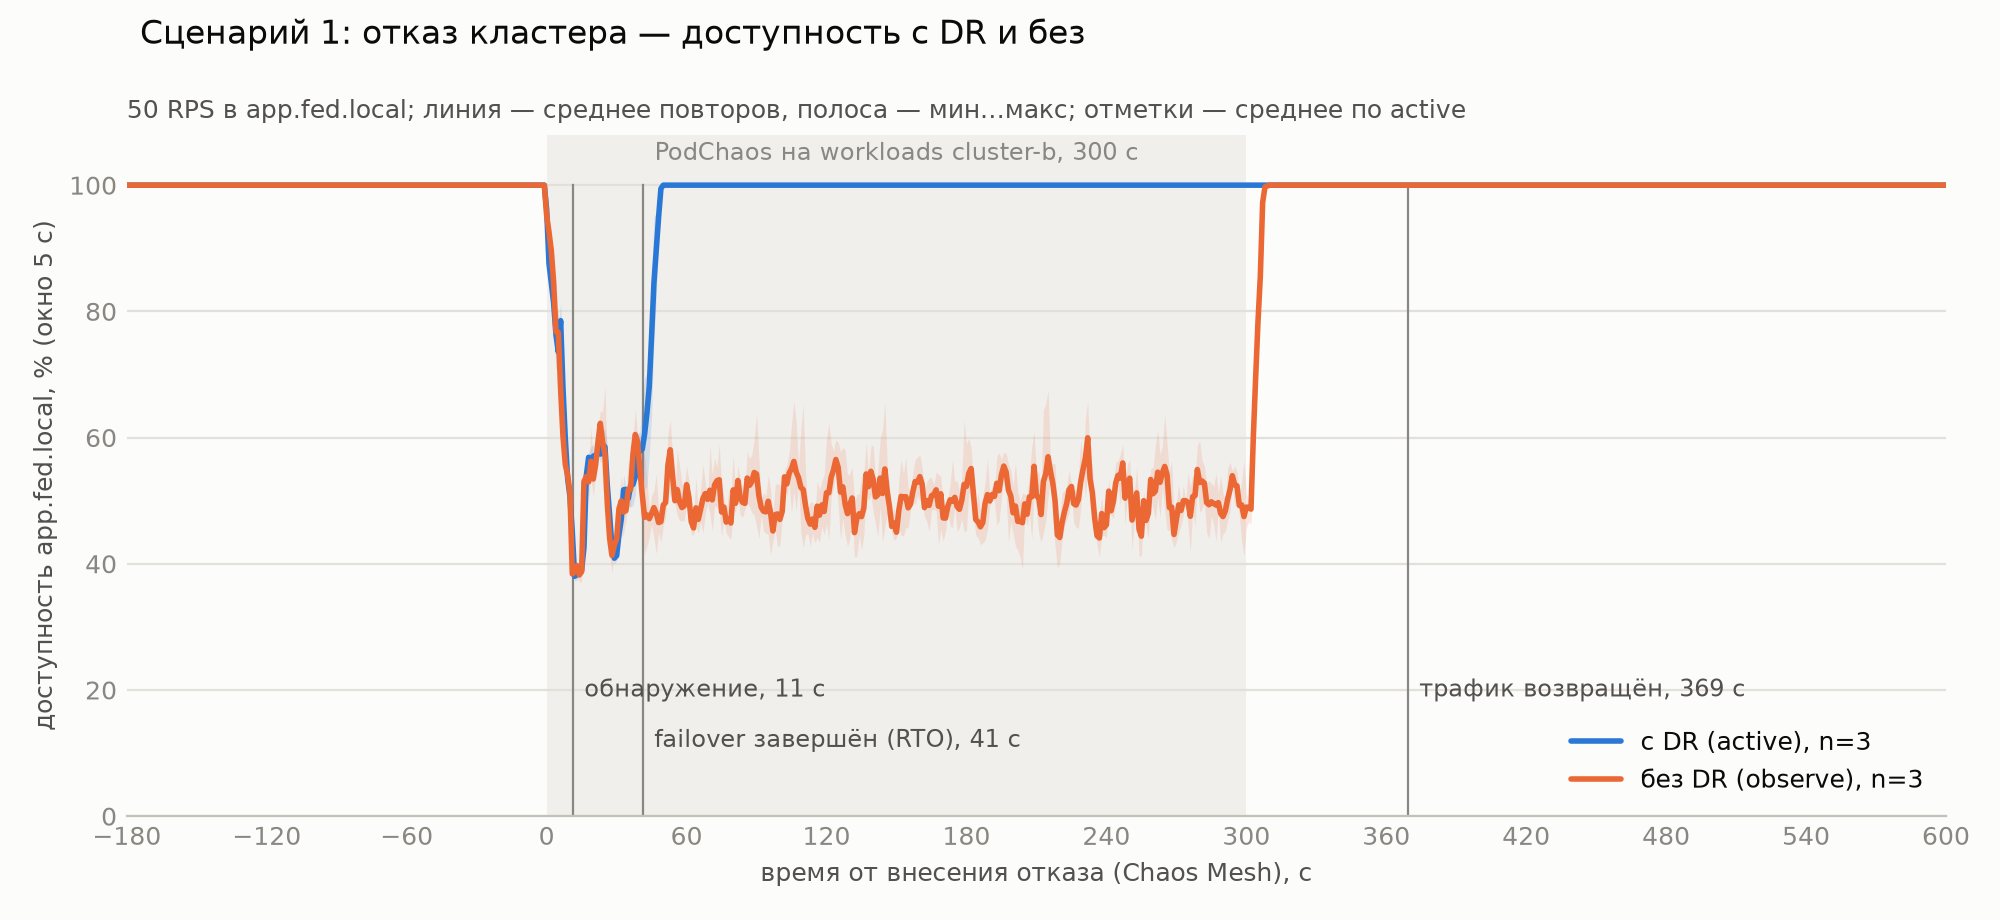
\includegraphics[width=\textwidth]{scenario1/task8-s1-availability.png}
  \caption{Доступность долгоживущего сервиса при отказе кластера с
  контроллером восстановления и без него (среднее трёх повторов)}
  \label{fig:s1}
\end{figure}

Снижение потерь по парам прогонов составило 86.8\%, 87.1\% и 87.3\%.
Оставшиеся потери приходятся на интервал от внесения отказа до переключения
трафика (около 41~с при половине трафика, направленной на отказавший
кластер). RTO складывается из времени обнаружения и 30~с подтверждения
отказа; эта задержка является платой за защиту от ложного переключения.

\section{Сценарий 2: деградация сети}

При разрабатываемом планировщике доля ошибок в окне отказа составила 2.40\%
против 4.41\% при наивном, то есть на 45.6\% меньше при цели не менее 20\%.
Разрабатываемый планировщик лучше наивного в каждой из трёх пар прогонов:
снижение составило 39.2\%, 50.5\% и 47.1\% (рис.~\ref{fig:s2}).

\begin{figure}[ht]
  \centering
  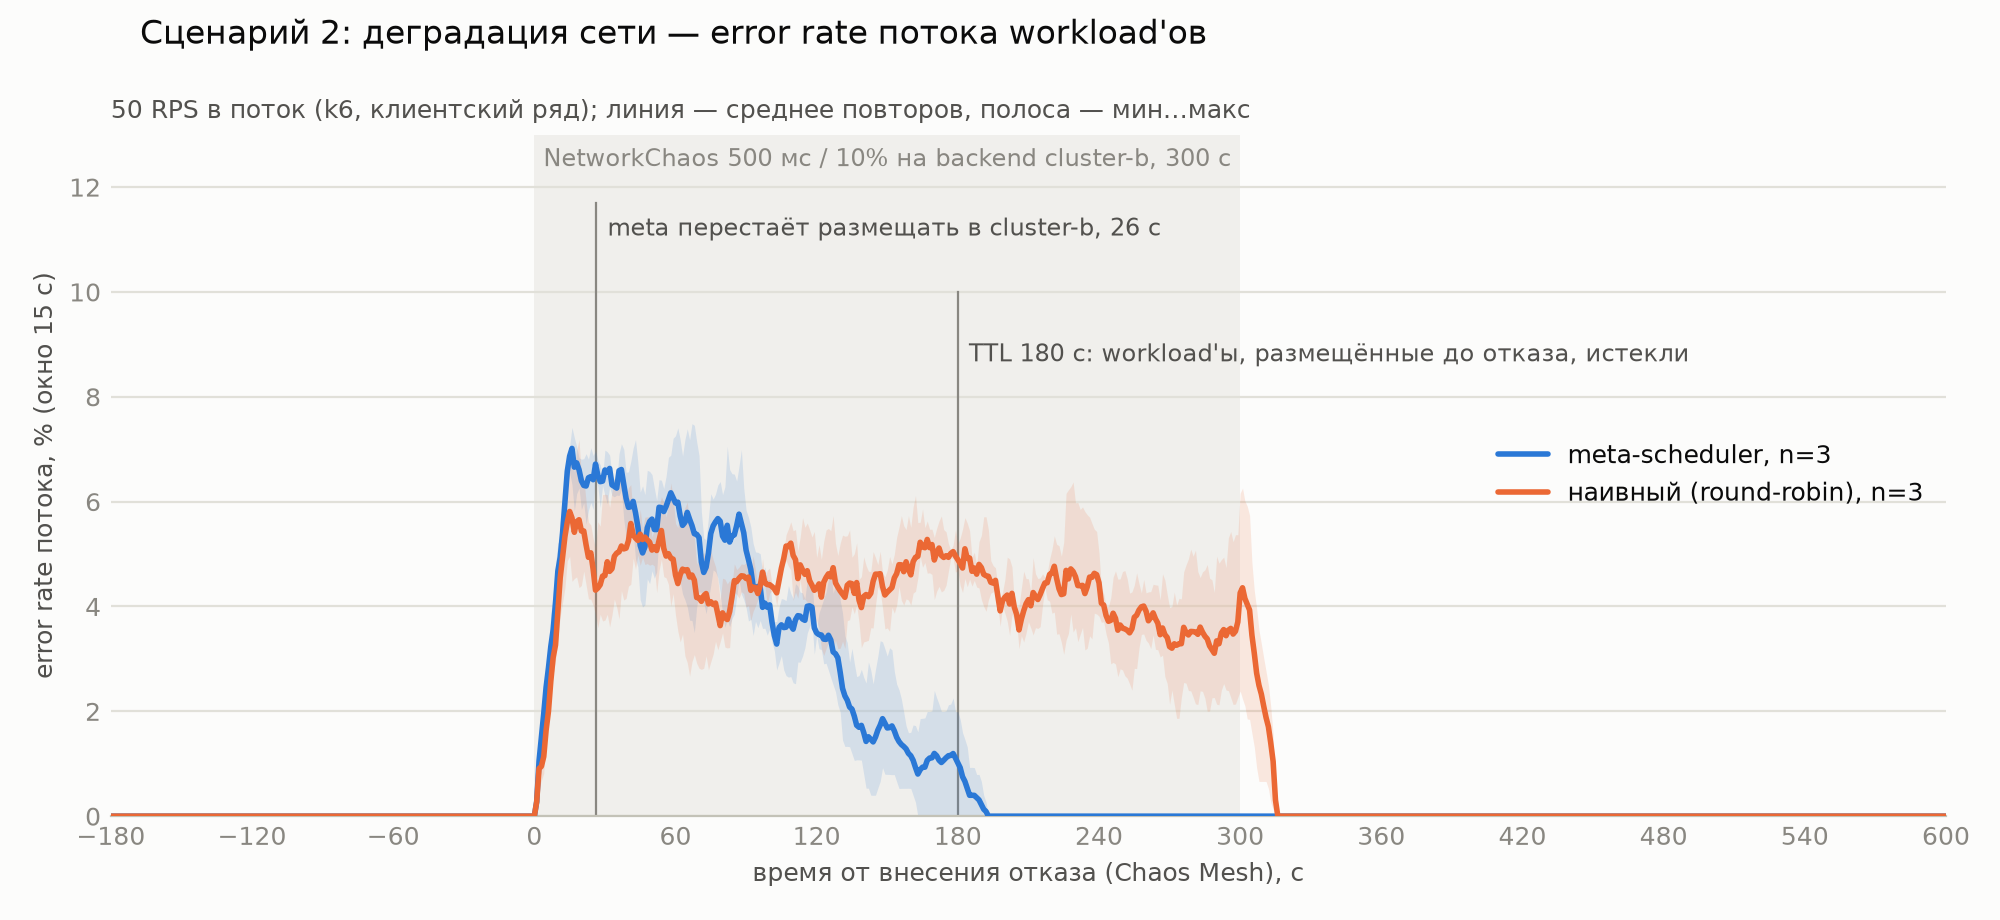
\includegraphics[width=\textwidth]{scenario2/task8-s2c-error-rate.png}
  \caption{Доля ошибок потока нагрузок при деградации сети в кластере B:
  разрабатываемый и наивный планировщики (среднее трёх повторов)}
  \label{fig:s2}
\end{figure}

Механизм эффекта виден по журналу решений: за время отказа разрабатываемый
планировщик не отправил в деградировавший кластер ни одного из 30
размещений, наивный~--- 15 из 29. Снижение оценки кластера в каталоге
наступает через 20--24~с после внесения отказа, первое решение в обход
деградировавшего кластера~--- через 25--27~с. Остаточные ошибки
разрабатываемого планировщика порождают нагрузки, размещённые в кластере B до
отказа: планировщик влияет только на новые размещения и не переносит уже
размещённые. Поэтому в первые 180~с отказа, пока эти нагрузки не завершились,
снижение составляет лишь 15.3\% (4.00\% против 4.72\%), а затем ошибки
разрабатываемого планировщика практически исчезают. Серверный ряд совпадает
с клиентским с точностью до 0.1 процентного пункта.

Кроме того, у наивного планировщика 5 из 87 размещений не перешли в
готовое состояние, у разрабатываемого~--- 0 из 87. Этот вред доля ошибок не
отражает, поскольку на неготовую нагрузку трафик не направляется.

\section{Сценарий 3: нарушение политики}

В режиме контроля не размещён ни один из 15 нарушителей, и каждая попытка
записана в журнал с корректным перечнем допустимых кластеров
(табл.~\ref{tab:s3}).

\begin{table}[ht]
  \centering
  \caption{Сценарий 3: три прогона по пять попыток}
  \label{tab:s3}
  \small
  \begin{tabularx}{\textwidth}{@{}>{\raggedright\arraybackslash}Xcccc@{}}
    \toprule
    Режим политик & Отклонено & Размещено & В журнале & \makecell{Задержка фиксации,\\медиана / макс.} \\
    \midrule
    Контроль & 15 из 15 & 0 & 15 & 4.7 / 9.9 с \\
    Аудит & 0 из 15 & 15 & 15 & 3.3 / 9.4 с \\
    Аудит, фиксация через отчёты политик & 0 из 15 & 15 & 15 & 3.3 / 30.2 с \\
    \bottomrule
  \end{tabularx}
\end{table}

Задержка фиксации нарушения ограничена периодом опроса (10~с). Фиксация через
отчёты политик медленнее: отчёт появляется в среднем через 23~с после
события Kyverno.

\section{Чувствительность к весам оценки}

Решения планировщика пересчитаны офлайн по записанным снимкам метрик для 66
точек симплекса весов с шагом 0.1 (181 решение, из них 59 в окне отказа).
Пересчёт совпадает с оценками планировщика с точностью $10^{-9}$. При
базовых весах доля размещений в деградировавший кластер равна 0\%, у
наивного планировщика~--- 51.7\%. Разрабатываемый планировщик лучше
наивного в 64 из 65 точек с $w_1 + w_2 > 0$ (рис.~\ref{fig:sensitivity}).
Единственное исключение~--- веса $(0.1, 0.0, 0.9)$: почти весь вес
приходится на загрузку, задержка не учитывается, и доля размещений в
деградировавший кластер составляет 59.3\%.

\begin{figure}[ht]
  \centering
  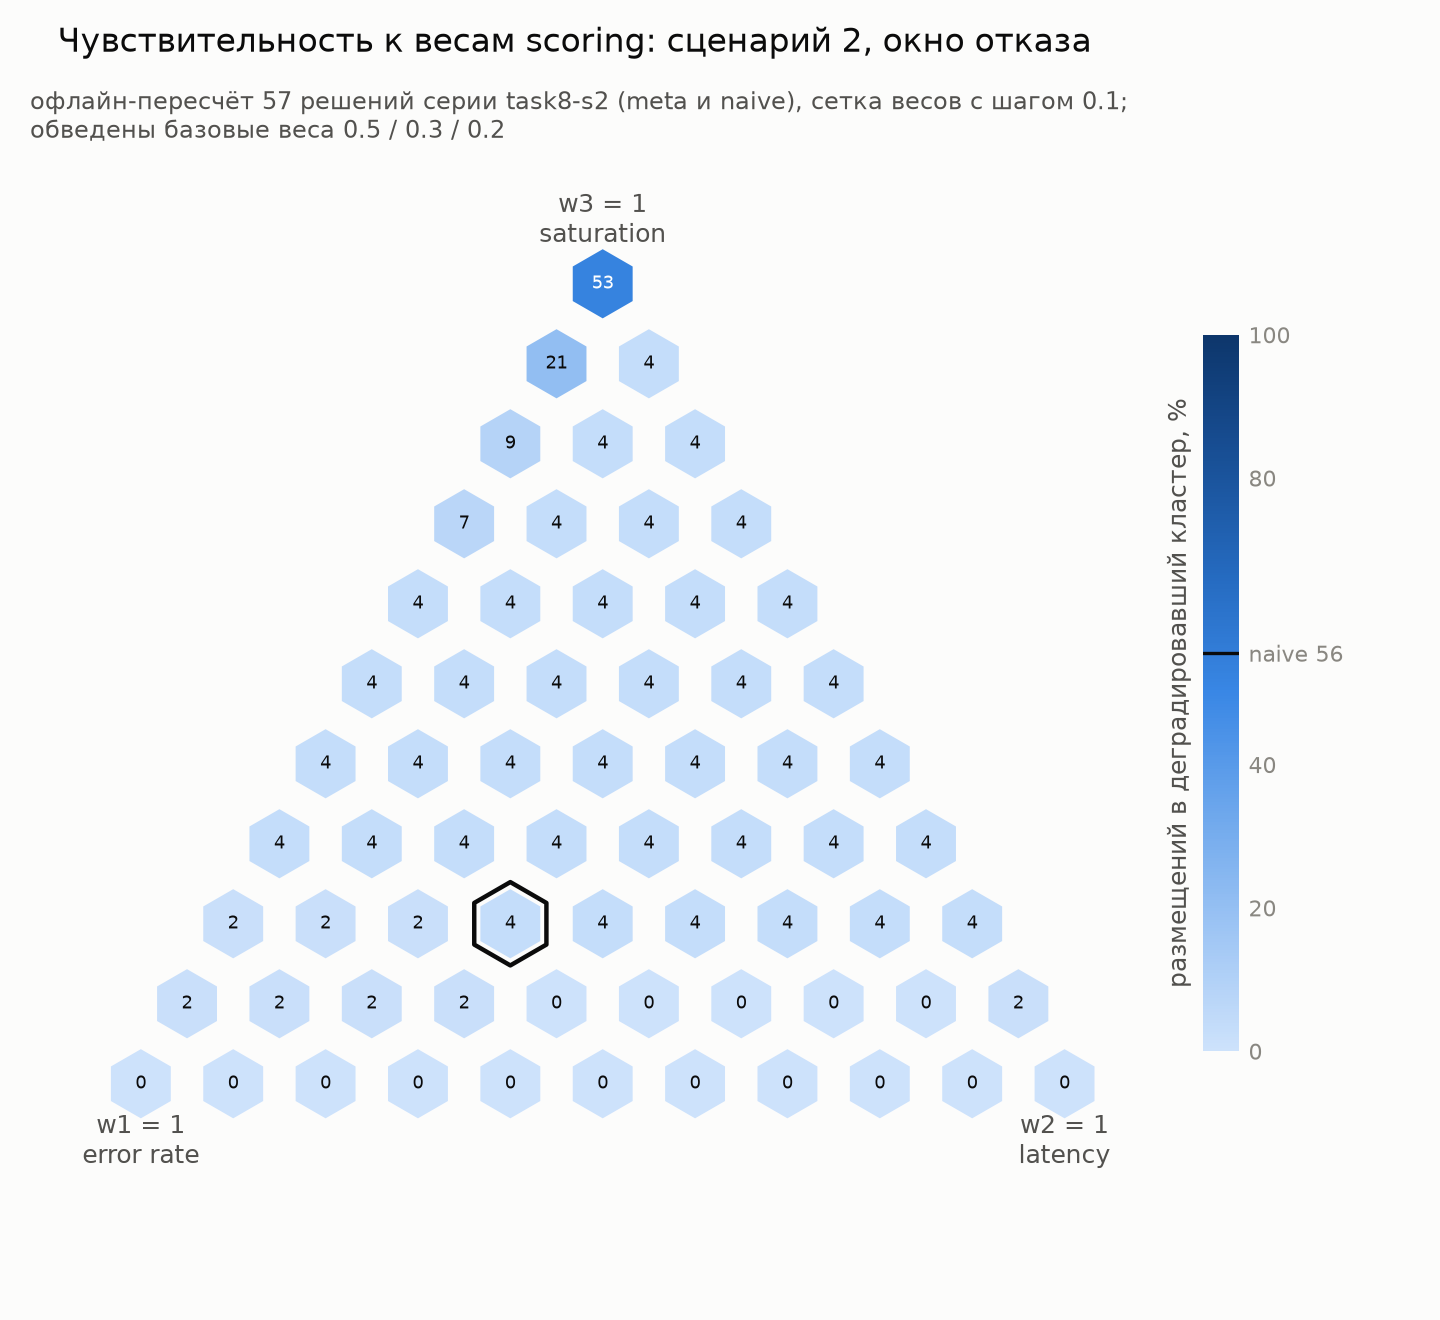
\includegraphics[width=0.75\textwidth]{task9/sensitivity.png}
  \caption{Доля размещений в деградировавший кластер в зависимости от весов
  оценки; обведены базовые веса}
  \label{fig:sensitivity}
\end{figure}

\section{Сравнение с другими методами выбора кластера}

\todo{Сравнение с другими методами выбора кластера: случайный выбор, выбор
по наименьшей загрузке, пороговый фильтр деградировавших кластеров~---
офлайн-пересчёт по записанным снимкам метрик (доля размещений в
деградировавший кластер). Раздел будет написан после проведения анализа.}

\section{Трассировка}

При доле записываемых трейсов 10\% собраны полные трейсы для 903--907 из
9000 запросов прогона. В штатном режиме серверная часть запроса занимает
около 0.5~мс по медиане: шлюз~--- 0.1~мс, переход из управляющего кластера в
кластер федерации~--- 0.2~мс, frontend~--- 0.04~мс, сеть до backend~---
0.14~мс. Накладные расходы трассировки неразличимы на фоне шума стенда:
медиана клиентской задержки составляет 0.83--1.03~мс при доле
записываемых трейсов 0\%, 10\% и 100\%, тогда как p95 между повторами одного
режима меняется от 2.3 до 6~мс.

\section{Достоверность данных каталога}

Снимки метрик, по которым принимал решения планировщик, сверены с рядами
Prometheus (732 снимка): доля ошибок совпадает в пределах 1 процентного
пункта в 98.1\% случаев, задержка p95 в пределах 10\%~--- в 99.6\% случаев.
Расхождения приходятся на моменты внесения и снятия отказа, когда ряд
изменяется на единицы процентных пунктов за 10~с: каталог получает данные в
реальном времени, а выгрузка выполняется позже по полным данным.
